% PREÁMBULO
\documentclass[letterpaper]{article}
\usepackage[utf8]{inputenc}
\usepackage[spanish]{babel}

\usepackage{enumitem}
\usepackage{titling}

% Símbolos
	\usepackage{amsmath}
	\usepackage{amssymb}
	\usepackage[utf8]{inputenc}
	\usepackage[T1]{fontenc}
	\usepackage{mathtools}
	\usepackage{multicol}
	\usepackage[thinc]{esdiff}

% Márgenes
	\usepackage
	[
		margin = 1.4in
	]
	{geometry}

% Imágenes
	\usepackage{float}
	\usepackage{graphicx}
	\graphicspath{{imagenes/}}
	\usepackage{subcaption}

% Ambientes
	\usepackage{amsthm}

	\theoremstyle{definition}
	\newtheorem{ejercicio}{Ejercicio}

	\newtheoremstyle{lemathm}{4pt}{0pt}{\itshape}{0pt}{\bfseries}{ --}{ }{\thmname{#1}\thmnumber{ #2}\thmnote{ (#3)}}
	\theoremstyle{lemathm}
	\newtheorem{lema}{Lema}

	\newtheoremstyle{lemademthm}{0pt}{10pt}{\itshape}{ }{\mdseries}{ --}{ }{\thmname{#1}\thmnumber{ #2}\thmnote{ (#3)}}
	\theoremstyle{lemademthm}
	\newtheorem*{lemadem}{Demostración}

% Ajustes
	\allowdisplaybreaks	% Los align pueden cambiar de página

% Macros
	\newcommand{\sumi}[2]{\sum_{i=#1}^{#2}}
	\newcommand{\dint}[2]{\displaystyle\int_{#1}^{#2}}
	\newcommand{\inte}[2]{\int_{#1}^{#2}}
	\newcommand{\dlim}{\displaystyle\lim}
	\newcommand{\limxinf}{\lim_{x\to\infty}}
	\newcommand{\limninf}{\lim_{n\to\infty}}
	\newcommand{\dlimninf}{\displaystyle\lim_{n\to\infty}}
	\newcommand{\limh}{\lim_{h\to0}}
	\newcommand{\ddx}{\dfrac{d}{dx}}
	\newcommand{\txty}{\text{ y }}
	\newcommand{\txto}{\text{ o }}
	\newcommand{\Txty}{\quad\text{y}\quad}
	\newcommand{\Txto}{\quad\text{o}\quad}
	\newcommand{\si}{\text{si}\quad}

	\newcommand{\etiqueta}{\stepcounter{equation}\tag{\theequation}}
	\newcommand{\tq}{:}
	\renewcommand{\o}{\circ}
	% \newcommand*{\QES}{\hfill\ensuremath{\boxplus}}
	% \newcommand*{\qes}{\hfill\ensuremath{\boxminus}}
	% \newcommand*{\qeshere}{\tag*{$\boxminus$}}
	% \newcommand*{\QESHERE}{\tag*{$\boxplus$}}
	\newcommand*{\QES}{\hfill\ensuremath{\blacksquare}}
	\newcommand*{\qes}{\hfill\ensuremath{\square}}
	\newcommand*{\QESHERE}{\tag*{$\blacksquare$}}
	\newcommand*{\qeshere}{\tag*{$\square$}}
	\newcommand*{\QED}{\hfill\ensuremath{\blacksquare}}
	\newcommand*{\QEDHERE}{\tag*{$\blacksquare$}}
	\newcommand*{\qel}{\hfill\ensuremath{\boxdot}}
	\newcommand*{\qelhere}{\tag*{$\boxdot$}}
	\renewcommand*{\qedhere}{\tag*{$\square$}}

	\newcommand{\abs}[1]{\left\vert#1\right\vert}
	\newcommand{\suc}[1]{\left(#1_n\right)_{n\in\N}}
	\newcommand{\en}[2]{\binom{#1}{#2}}
	\newcommand{\upsum}[2]{U(#1,#2)}
	\newcommand{\lowsum}[2]{L(#1,#2)}

	\newcommand{\N}{\mathbb{N}}
	\newcommand{\Q}{\mathbb{Q}}
	\newcommand{\R}{\mathbb{R}}
	\newcommand{\Z}{\mathbb{Z}}
	\newcommand{\eps}{\varepsilon}
	\newcommand{\ttF}{\mathtt{F}}
	\newcommand{\bfF}{\mathbf{F}}

	\newcommand{\To}{\longrightarrow}
	\newcommand{\mTo}{\longmapsto}
	\newcommand{\ssi}{\Longleftrightarrow}
	\newcommand{\sii}{\Leftrightarrow}
	\newcommand{\then}{\Rightarrow}

	\newcommand{\pTFC}{{\itshape 1er TFC\/}}
	\newcommand{\sTFC}{{\itshape 2do TFC\/}}

%Code

	\usepackage{listings}
	\usepackage{xcolor}
	\lstset { %
		language=C++,
		backgroundcolor=\color{black!5}, % set backgroundcolor
		basicstyle=\footnotesize,% basic font setting
		breaklines=true
		postbreak=\mbox{\textcolor{red}{$\hookrightarrow$}\space}
	}

% Membrete
	\usepackage{fancyhdr}
	\setlength{\headheight}{14pt}
	\pagestyle{fancy}
	\fancyhf{}
	\rhead{\theauthor}
	\lhead{\thetitle}
	\cfoot{\thepage}

% Datos
    \title{Estructuras y Algoritmos II\\Set de problemas II}
    \author{Rubén Pérez Palacios\\Profesora: Dra. Claudia Elvira Esteves Jaramillo}
    \date{3 Junio 2020}

% DOCUMENTO
\begin{document}
	\maketitle

	\section*{Problemas}

	\begin{enumerate}
		\item El Herr Professor Doktor Georg von den Dschungel tiene un \'arbol binario de 23 nodos en los que cada noto est\'a etiquetado con una letra \'unica del alfabeto alem\'an (incluye las letras {\"A}, {\"O}, {\"U} y {\ss} que no hay que confundir con A, O, U y B). Los recorridos en preorden y postorden de los nodos del \'arbol son :

		\begin{itemize}
		\item[]{Preorden: B~K~\"U~E~H~L~Z~I~\"O~R~C~\ss~T~S~O~A~\"A~D~F~M~N~U~G}
		\item[]{Postorden: H~I~\"O~Z~R~L~E~C~\"U~S~O~T~A~\ss~K~D~M~U~G~N~F~\"A~B}
		\end{itemize}
		
		Dibuja el \'arbol del Herr Professor Doktor von den Dschungel.

		\begin{figure}[H]
			\centering
			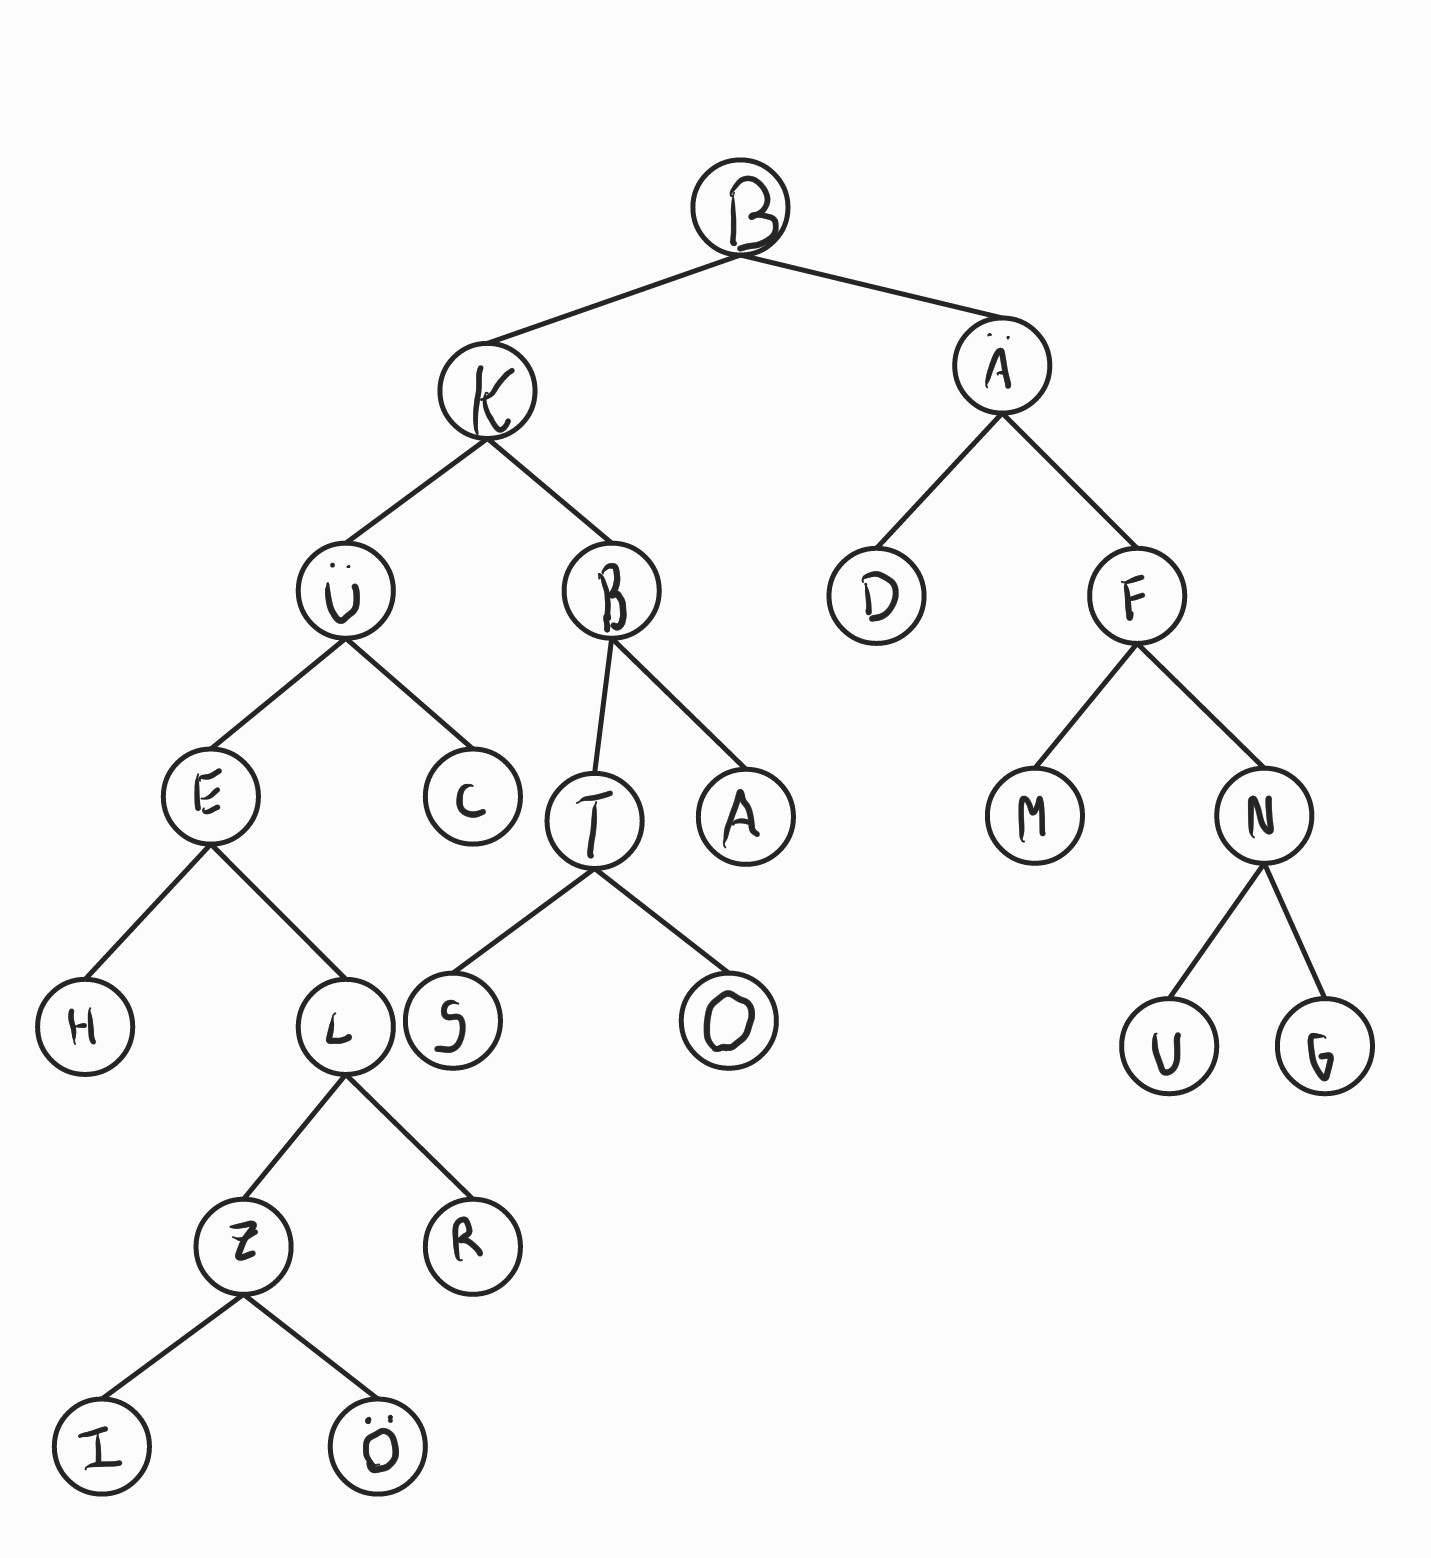
\includegraphics[scale=.25]{images/arbol}
		\end{figure}

		\item ¿Cuales son el número mínimo y máximo de nodos en un árbol binario completo de altura $h$.
		
		EL número minimo de nodos es de $2^h$ y el máximo es de $2^{h+1} - 1$.
		

		\item ¿Cuales son la propiedades de un árbol rojo-negro?
		
		\begin{itemize}
			\item Todo nodo es negro o rojo.
			\item La raíz es negra
			\item Todas la hojas especiales son negras (estas son agregadas a todos los nodos hojas que no son especiales)
			\item Si un nodo es rojo entonces sus negros.
			\item Todo camino de un nodo a sus hojas especiales tienen la misma cantidad de hojas negras.
		\end{itemize}
		
		\item ¿Cuál es la complejidad (en notación asintótica) de construir un árbol rojo-negro de n nodos?
		
		Las operaciones que tomaria construir el arbol serían

		\[\sum_{i=0}^{N-1} log(i) = log((N-1)!)\]

		puesto que nos interesa solo la notación $O$ ignoraremos el $-1$, luego

		\[log(N!) \leq log(N^N) = Nlog(N)\].

		Ahora veamos que para $N \geq 4$

		\[N! \geq N^{\frac{N}{4}},\]

		por lo que

		\[\frac{Nlog(N)}{log(N!)} \leq \frac{Nlog(N)}{log(N^{\frac{N}{4}})} = 4,\]

		por definición de la notación $O$ concluimos que la complejidad de construir un árbol de $N$ nodos es

		\[O(Nlog(N))\]

		\item ¿Cuál es la ventaja de utilizar un árbol rojo-negro en lugar de un árbol binario general?
		
		Al ser autobaleanceado las operaciones en el se puede hacer en $O(log(N))$, mientras que en un arbol binario serían en $O(N)$, ejemplo buscar un elemento.

		\newpage

		\item Árbol rojo-negro
		
		\begin{enumerate}
			\item Inserta 41, 38, 31, 12, 19, 8.
			
				\begin{figure}[H]
					\centering
					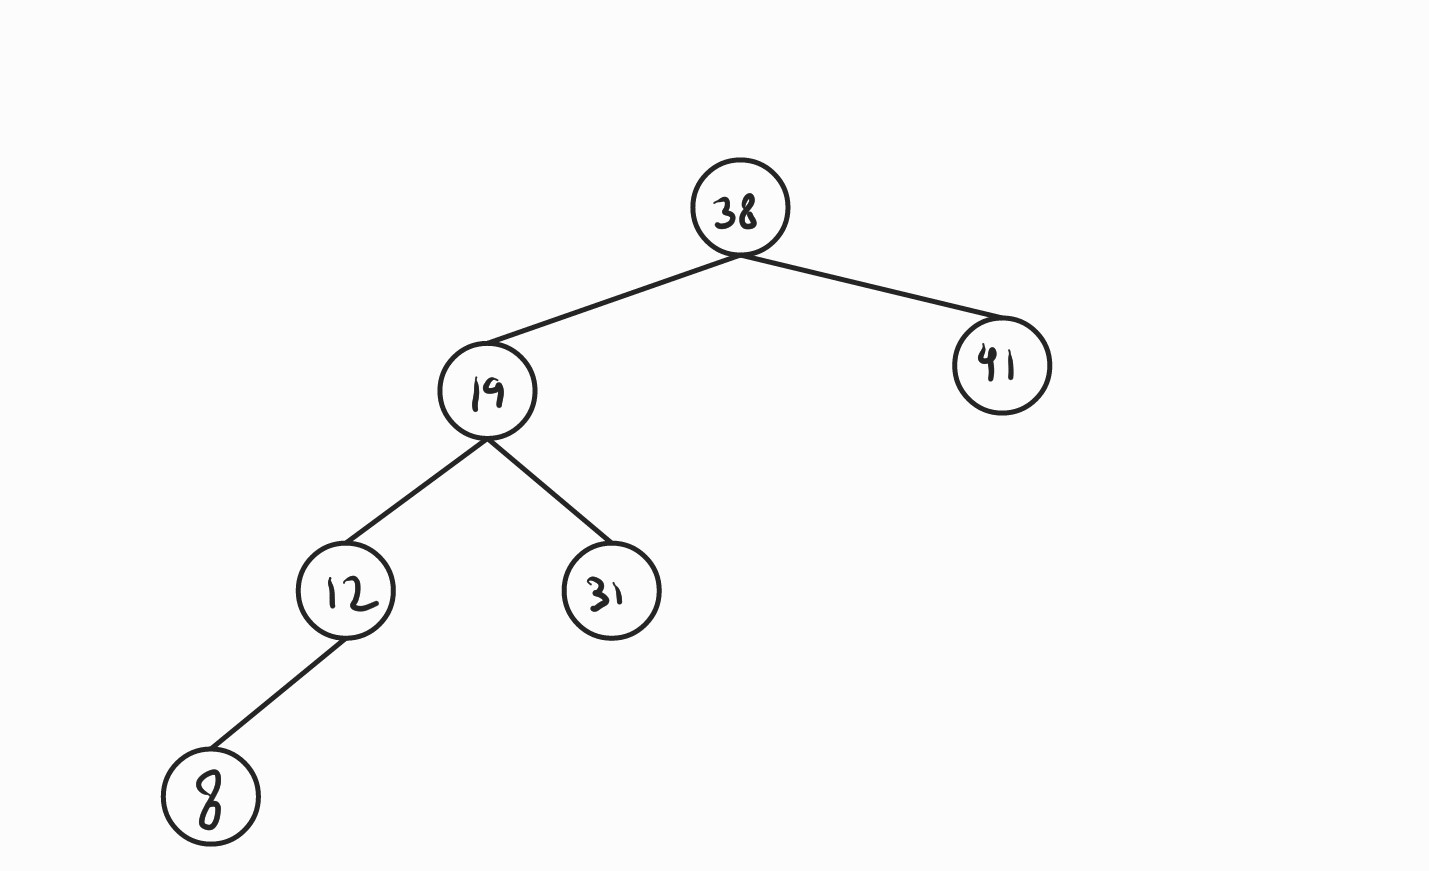
\includegraphics[scale=.25]{images/arbol2}
				\end{figure}

			\item Elimina 8, 12, 19.
			
				\begin{figure}[H]
					\centering
					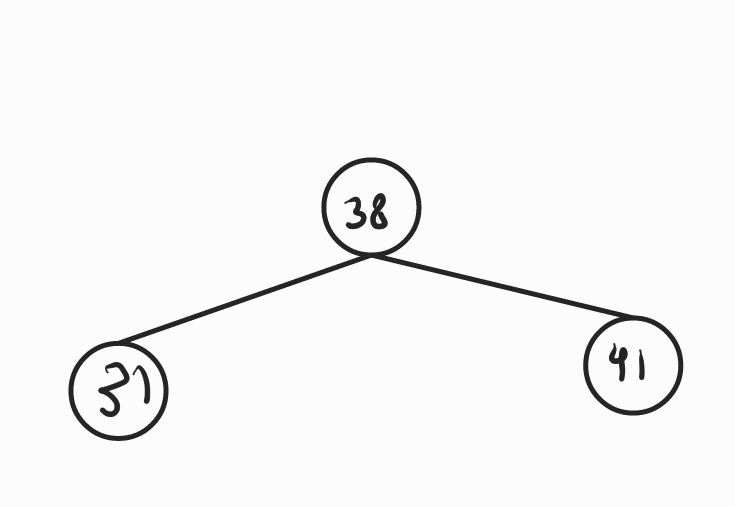
\includegraphics[scale=.25]{images/arbol3}
				\end{figure}

		\end{enumerate}

		\item No se puede ya que de ser así se podria tener un algoritmo de ordenamiento con \linebreak $O(Nlog^2(N))$ puesto que esto es imposible ya que lo mas rapido posible en una algoritmo de ordenamiento de comparación es $O(NlogN)$ (se dumuestra con un arbol de decisiones).
		
		\item Ilustra cada paso del COUNTING-SORT en el arreglo $A = \{6,0,2,0,1,3,4,6,1,3,2\}$.
		
		Primero cuenta cuantos hay de cada uno
		
		\begin{tabular}{|c|c|c|c|c|c|c|}
			\hline
			0 & 1 & 2 & 3 & 4 & 5 & 6\\
			\hline
			2 & 2 & 2 & 2 & 1 & 0 & 2\\
			\hline
		\end{tabular}

		Luego hacemos sumas parciales sobre este arreglo

		\begin{tabular}{|c|c|c|c|c|c|c|}
			\hline
			0 & 1 & 2 & 3 & 4 & 5 & 6\\
			\hline
			2 & 4 & 6 & 8 & 9 & 9 & 11\\
			\hline
		\end{tabular}

		Obtenemos el orden sobre este arreglo, ya que el indice representan los elementos de nuestro arreglo original y sus valores representan la posición en la que deben ir, cada vez que pases por uno deberas restarle 1 a ese valor para que si hay otro igual a ti se actualice su posición.

		\begin{tabular}{|c|c|c|c|c|c|c|c|c|c|c|}
			\hline
			0 & 0 & 1 & 1 & 2 & 2 & 3 & 3 & 4 & 6 & 6\\
			\hline
		\end{tabular}

		\item Apartir de tu geolocalización de tu telefono podrías construir un grafo donde cada persona es un nodo y entre dos nodos hay una arista si sus telefonos estuvieron a una distancia muy cercana (habría que definir bien que significa cercana). Así cuando se detecte que alguien tiene COVID, inmediatamente todos sus vecinos inmediatos en el grafo son sospechosos (no se me ocurre otra palabra, a lo mejor propensos) a haber contraido el virus. De esta forma se podría hacer una investigación y seguimiento de los casos, para así controlar la expansión de este. Es importante mencionar que los datos recolectados por la geolocalización deberán de ser utilizados únicamente para construir el arbol.

	\end{enumerate}
	

\end{document}